\documentclass[Main]{subfiles}
\begin{document}

\textbf{Classifier accuracy}

The classifier accuracy is tested on feature sets, extracted from the collected data, that weren't used for training. The accuracy of the classifier varies from each training, since the data is shuffled before some of the data is selected for training. However, the accuracy lies around 0.94-0.95. This very high accuracy, is undoubtedly a result of, two thirds of the training and test data, being queried with emoticons, which in this case is a very informative feature. The 10 most informative features for one training session show below:

\begin{figure}[h]
  \centering
  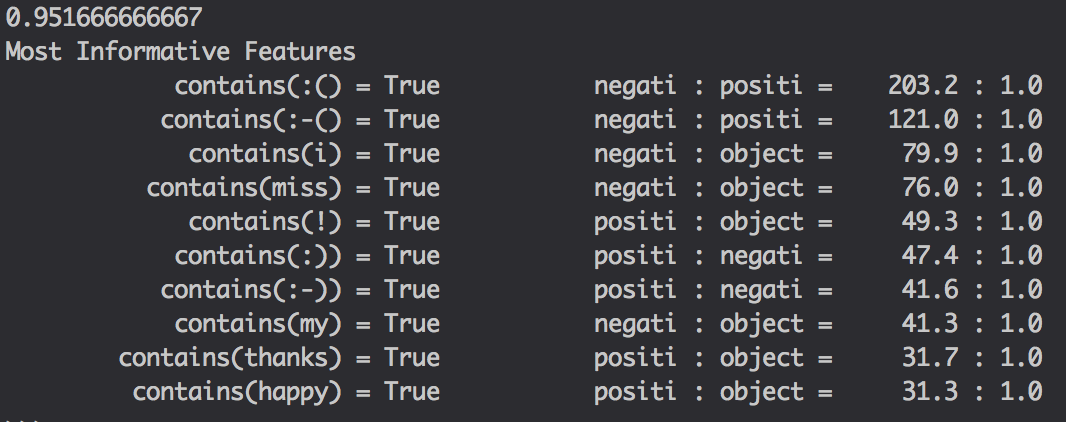
\includegraphics[width=0.485\textwidth]{accuracy.png}
  \caption{Accuracy and most informative features}
  \label{fig:accuracy}
\end{figure}


\textbf{General}

The application as a whole can be run through ``website.py'', 
which renders a web front-end on ``localhost:5000'' and gives the user access to querying tweets.
The front-end is shown on \autoref{fig:website}, where the hashtag ``\#python'' has been queried.

\begin{figure}[h]
  \centering
  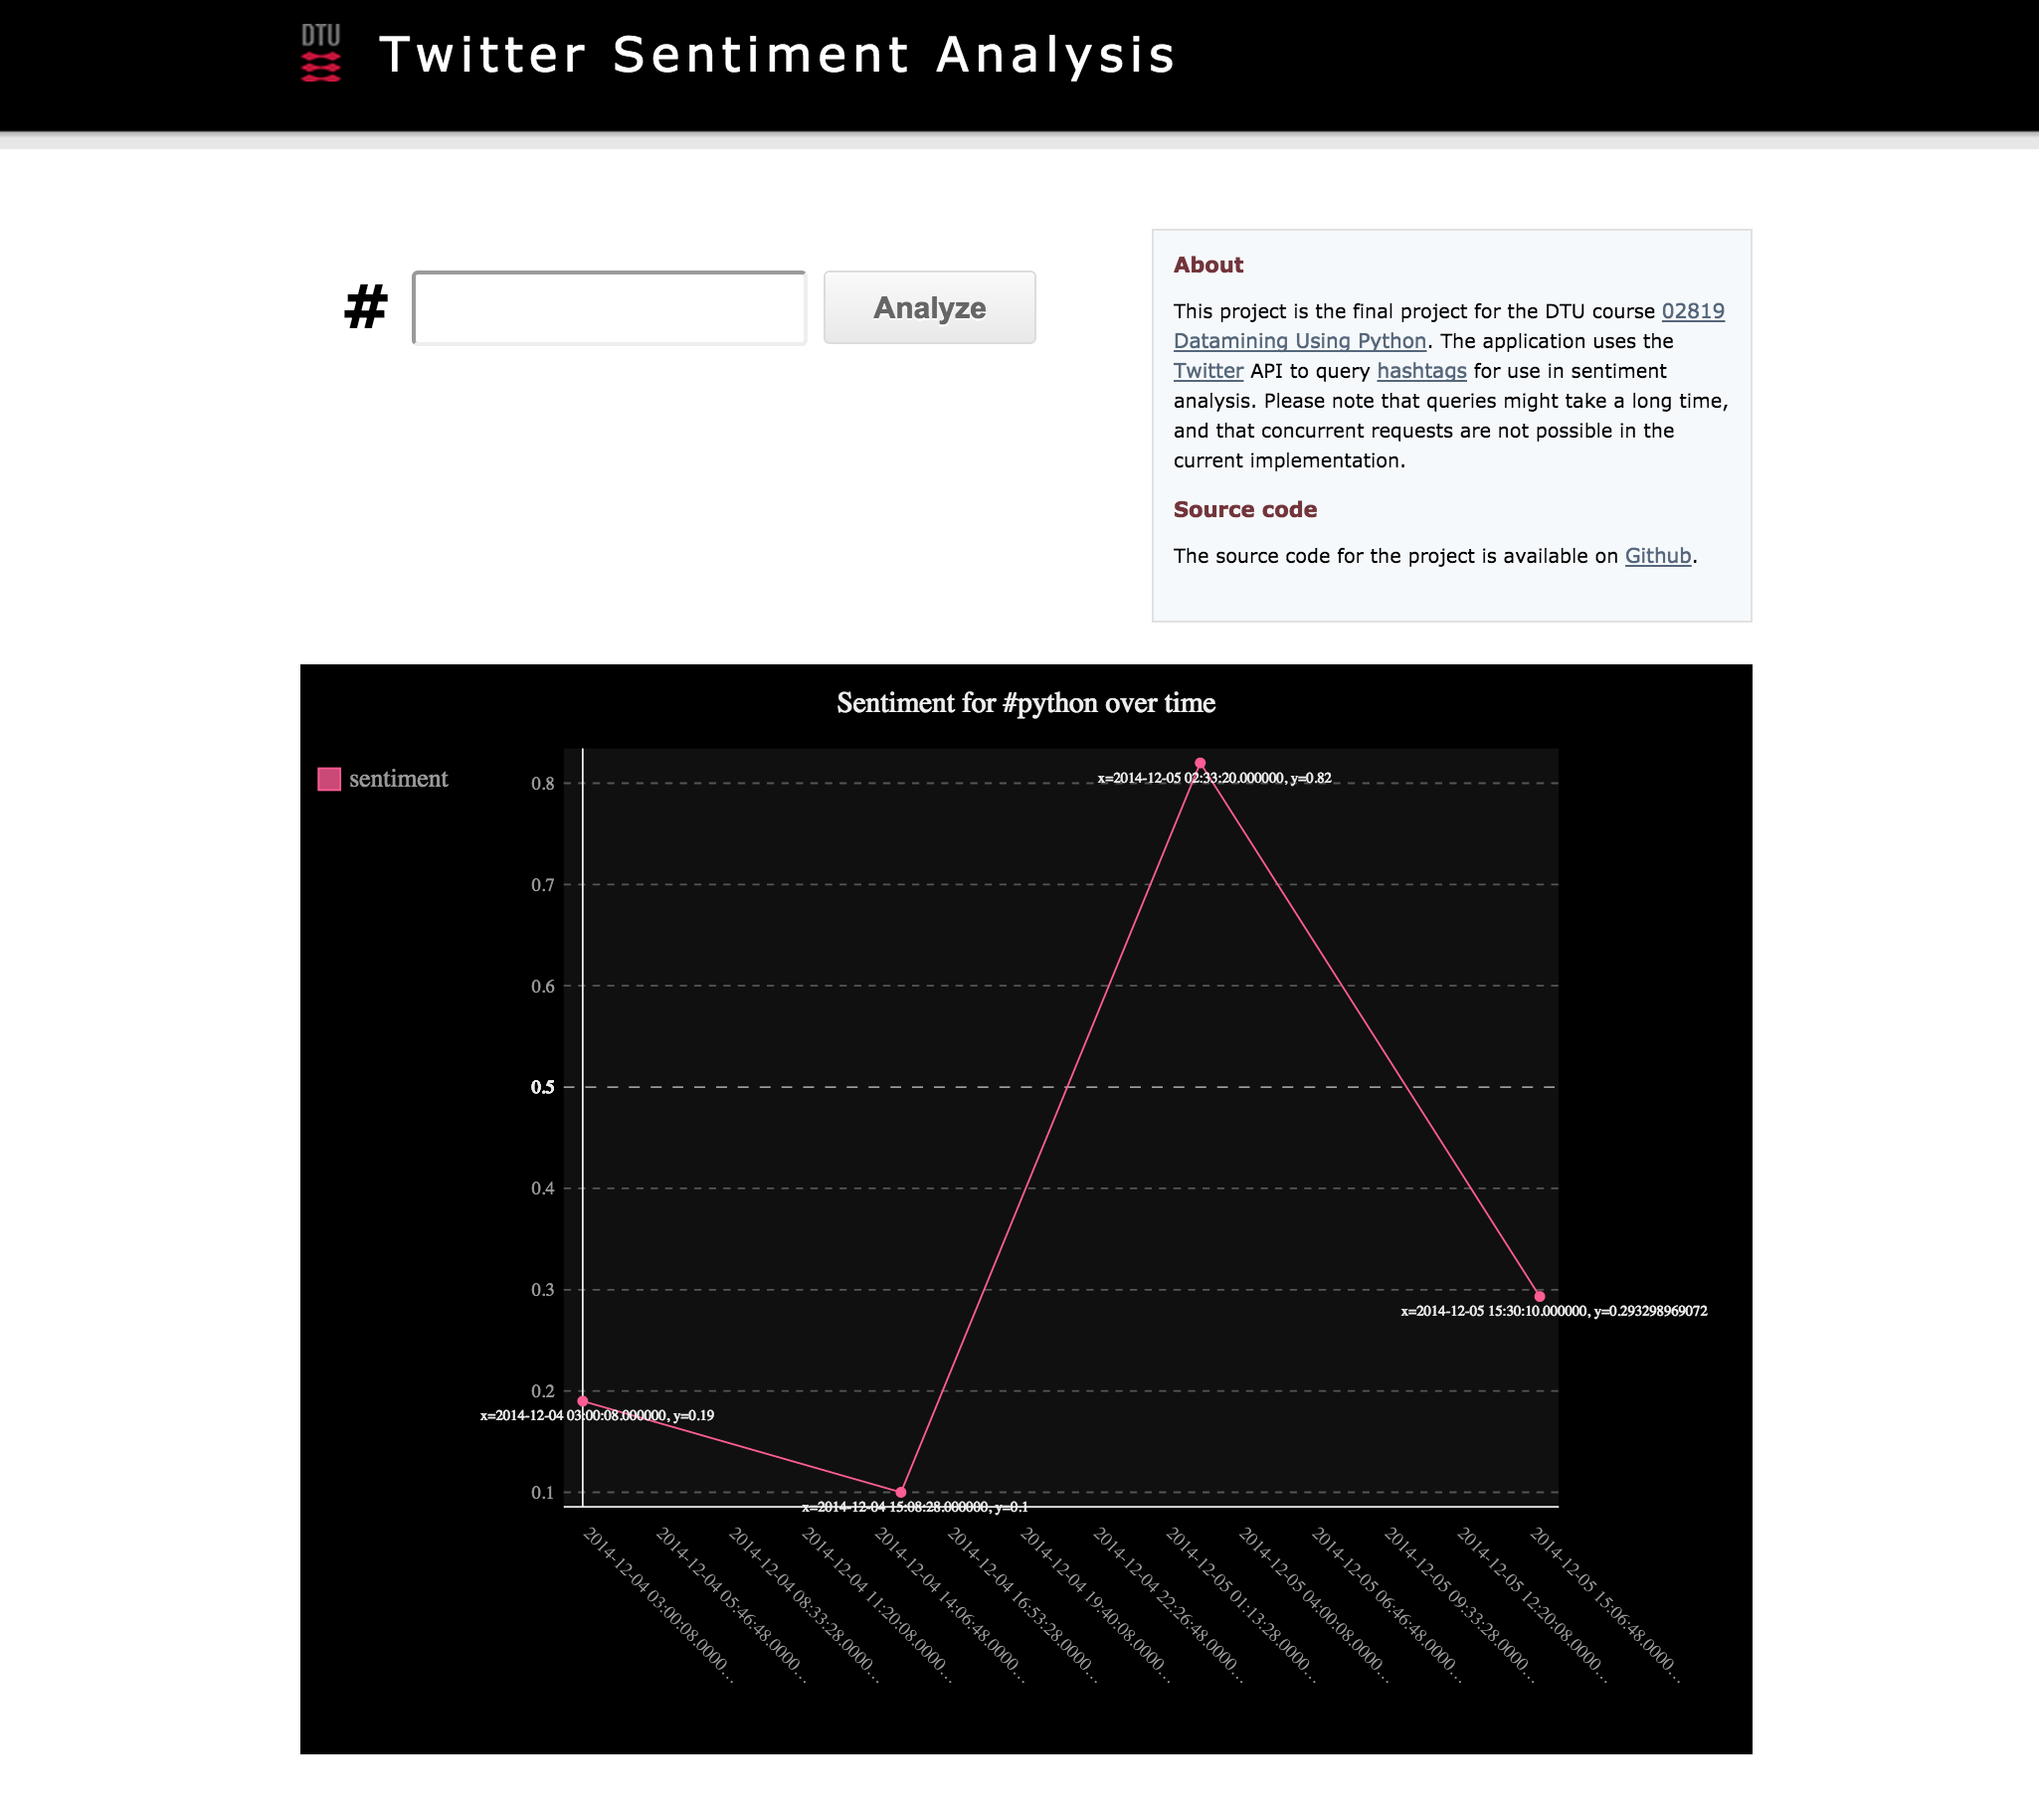
\includegraphics[width=0.485\textwidth]{website.png}
  \caption{Web-interface for the application}
  \label{fig:website}
\end{figure}

While the web-interface does look rather simplistic, there's a lot of moving parts behind it.
The steps for querying a hashtag are listed below:
\begin{enumerate}
\item Look up tweets using the Twitter API
\item De-serialize the tweet from JSON to the appropriate domain model
\item Extract the feature-set of the tweets
\item Analyze the sentiment polarity of the tweets
\item Insert the analyzed tweets into a PostgreSQL database
\item Render a graph of the analyzed tweets
\item Render the updated web-interface to the user
\end{enumerate}

One of the limitations of the current implementation, is that querying Twitter takes a relatively long period of time,
approximately 5 seconds per 100 tweets.
This makes it hard to get a very precise and dense result set, but it does give us an impression of how a more complete system would behave.

Testing of the application is done using ``nosetests'', which makes it easy to run tests and get a nicely formatted output.
While the test-coverage of the project isn't 100\%, experience in how to write tests for a Python project has been gained.


\end{document}
